\documentclass{article}
\usepackage{amsthm,hyperref,mathtools,mathpartir,cleveref,mathrsfs,amssymb,url,paralist,xspace,braket,ifmtarg}
\usepackage[status=draft]{fixme}
\newtheorem{thm}{Theorem}[section]
\crefname{thm}{Theorem}{Theorems}
\newtheorem{lem}[thm]{Lemma}
\crefname{lem}{Lemma}{Lemmas}
\newtheorem{cor}[thm]{Corollary}
\crefname{cor}{Corollary}{Corollaries}
\theoremstyle{definition}
\newtheorem{defn}[thm]{Definition}
\crefname{defn}{Definition}{Definitions}
\newtheorem{defns}[thm]{Definitions}
\crefname{defns}{Definitions}{Definitions}
\newtheorem{eg}[thm]{Example}
\crefname{eg}{Example}{Examples}
\theoremstyle{remark}
\newtheorem{rmk}[thm]{Remark}
\crefname{rmk}{Remark}{Remarks}
\usepackage{tikz}
\usepackage{tikz-cd}
\usetikzlibrary{decorations.markings}
\tikzset{edge/.style={decoration={markings,mark=at position 0.5 with {\arrow{>}}},postaction={decorate}}}
\tikzset{vertex/.style={circle,draw,inner sep=1pt}}
\usetikzlibrary{shapes.geometric}
\tikzset{outer/.style={regular polygon,regular polygon sides=3,inner sep=1pt,draw,shape border rotate=180}}
\tikzset{houter/.style={regular polygon,regular polygon sides=3,inner sep=1pt,draw,shape border rotate=270}}
\tikzset{cross/.style={white,line width=3pt}}
\let\sto\looparrowright
\def\M{\mathcal{M}}
\def\A{\mathcal{A}}
\def\B{\mathcal{B}}
\def\C{\mathcal{C}}
\def\P{\mathcal{P}}
\def\Q{\mathcal{Q}}
\def\D{\mathcal{D}}
\def\G{\mathcal{G}}
\def\H{\mathcal{H}}
\def\K{\mathcal{K}}
\def\L{\mathcal{L}}
\def\R{\mathcal{R}}
% \def\Cat{\ensuremath{\mathcal{C}\mathit{at}}}
\let\setof\Set
\def\Set{\mathbf{Set}}
\def\Cat{\ensuremath{\mathbf{Cat}}}
\def\Fib{\mathcal{F}\mathit{ib}}
\def\Prof{\mathcal{P}\mathit{rof}}
\def\cpg{\ensuremath{\mathbf{CPG}}\xspace}
\def\dom{\mathrm{dom}}
\def\cod{\mathrm{cod}}
\def\id{\mathrm{id}}
\def\side#1{{\scriptstyle(#1)}}
\def\sid{\side{\id}}
% \def\twocell#1#2#3#4{\inferrule*[Left={$\side{#1}$},Right={$\side{#4}$}]{#2}{#3}}
% \def\twocelll#1#2#3#4{\inferrule*[left={$\side{#1}$},Right={$\side{#4}$}]{#2}{#3}}
% \def\twocellr#1#2#3#4{\inferrule*[Left={$\side{#1}$},right={$\side{#4}$}]{#2}{#3}}
% \def\twocelllr#1#2#3#4{\inferrule*[left={$\side{#1}$},right={$\side{#4}$}]{#2}{#3}}

\newcounter{nodemaker}
\setcounter{nodemaker}{0}
\def\twocell#1{%
  \global\edef\mynodeone{twocell\arabic{nodemaker}}%
  \stepcounter{nodemaker}%
  \global\edef\mynodetwo{twocell\arabic{nodemaker}}%
  \stepcounter{nodemaker}%
  \ar[#1,phantom,shift left=3,""{name=\mynodeone}]%
  \ar[#1,phantom,shift right=3,""'{name=\mynodetwo}]%
  \ar[Rightarrow,from=\mynodeone,to=\mynodetwo]%
}
\newcommand{\drpullback}[1][dr]{\ar[#1,phantom,near start,"\lrcorner"]}
\newcommand{\dlpullback}[1][dl]{\ar[#1,phantom,near start,"\llcorner"]}
\newcommand{\urpullback}[1][ur]{\ar[#1,phantom,near start,"\urcorner"]}
\newcommand{\ulpullback}[1][ul]{\ar[#1,phantom,near start,"\ulcorner"]}

\let\ot\leftarrow
\let\xto\xrightarrow
\let\xot\xleftarrow
\let\tot\leftrightarrow
\def\o{^{\circ}}
\tikzset{horiz/.style={"\mathclap\bullet" description}}
\def\genus{\mathsf{genus}}
\def\degree{\mathsf{degree}}
\def\rank{\mathsf{rank}}
\def\N{\mathbb{N}}
\def\Np{\N_{\bullet}}
\def\hy{\mathcal{H}\mathit{y}\mathcal{G}\mathit{ph}}
\def\hyrel{\mathcal{H}\mathit{y}\mathcal{R}\mathit{el}}
\def\thy{\mathcal{T}}
\def\dhy{\mathcal{D}}
\def\fhy{\mathcal{F}}
\def\ehy{\mathcal{E}\mathit{xt}\mathcal{H}\mathit{y}\mathcal{G}\mathit{ph}}

\makeatletter
\def\ins#1#2#3#4{#1 \underset{\@ifmtarg{#2}{#3}{#3\in #2}}{\circ} #4}
\def\insy{\circ}
\makeatother
\def\bE{\mathbf{E}}
\def\bC{\ensuremath{\mathbf{C}}\xspace}
\def\bS{\ensuremath{\mathbf{S}}\xspace}
\def\Ebar{\overline{\mathbf{E}}}
\def\Gbar{\overline{\mathcal{G}}}
\def\Cbar{\overline{\mathcal{C}}}
\def\Hbar{\overline{\mathcal{H}}}
\def\Kbar{\overline{\mathcal{K}}}
\def\Lbar{\overline{\mathcal{L}}}
\def\dhybar{\overline{\mathcal{D}}}

\def\ec{\diamond}
\def\edgectx{\;\mathsf{edgectx}}
\def\loopctx{\;\mathsf{loopctx}}
\def\vertex{\;\mathsf{vertex}}
\def\ctx{\;\mathsf{ctx}}
\def\graph{\;\mathsf{graph}}
\def\type{\;\mathsf{type}}
\let\types\vdash
\let\jdeq\equiv

\hyphenation{hyper-graph}
\hyphenation{hyper-graphs}

\title{Hypercategories and some kind of type theory}
\author{Dan Licata \and\ Mitchell Riley \and\ Patrick Schultz \and\ Michael Shulman}
\begin{document}
\maketitle

\section{Hypergraphs}
\label{sec:hypergraphs}

\begin{defn}
  A \textbf{hypergraph} is a span
  \[ V \ot F \to E \]
  in which $V$ and $F$ are sets, each fiber of the map $F\to V$ is a finite set equipped with a linear ordering, and $E$ is a groupoid all of whose objects have finitely generated free automorphism groups.

  The isomorphism classes of objects of $E$ are called \textbf{edges}, the elements of $V$ are called \textbf{vertices}, and those of $F$ are called \textbf{flags}.
  If a vertex and an edge are the image of a common flag, we say they are \textbf{incident}; thus the flags are the ``witnesses of incidence''.
  We also speak of a flag as being \textbf{incident} to its associated edge and vertex.
\end{defn}

We allow vertices that are not incident to any edges, and edges that are not incident to any vertices.
Also a vertex and an edge can be ``incident more than once'', i.e.\ the image of more than one common flag.

\begin{defn}
  Let $\G=(V\ot F\to E)$ be a hypergraph.
  \begin{itemize}
  \item The \textbf{degree} of a vertex in $\G$ is the cardinality of the set of flags adjacent to it, which is a natural number.
    The \textbf{rank} of an edge in $\G$ is the cardinality of the set of flags adjacent to it, which in general can be finite or infinite.
    We say $\G$ %has \textbf{finite rank} if all its ranks are finite, and $\G$
    is \textbf{finite} if it has finitely many vertices and edges (hence also finitely many flags).
  \item The free rank of the automorphism group of an edge is called its \textbf{genus}.
    We say $\G$ has \textbf{genus zero} if all of its edges have genus zero, i.e.\ $E$ is equivalent to a discrete set.
  \item The \textbf{connected components} of $\G$ are the connected components of the groupoid pushout of the span $V \leftarrow F \to E$.
    We say $\G$ is \textbf{connected} if it has exactly one connected component.
    % In particular, vertices not incident to any edges, and edges not incident to any vertices, lie in their own connected components.
  \item We say $\G$ is \textbf{simple} if no edge is incident to any vertex more than once, so that the span $E \ot F \to V$ is a relation.
  \end{itemize}
\end{defn}

The (directed) hypergraphs of~\cite{glpn:directed-hypergraphs} are our (directed) finite simple hypergraphs of genus zero, but without the orderings on the flags adjacent to each vertex.
We include the orderings because we eventually want a correspondence to linear syntax, and to definitions of prop and polycategory using ordered lists of objects, but they are not essential to the theory.
We draw vertices as dots and edges as lines connecting them, which are allowed to ``branch'' in order to connect more than two vertices.
We draw an edge of positive genus as containing ``loops''.
\fxnote{Add some examples.}

\begin{defn}
  A \textbf{morphism of hypergraphs} is a diagram
  \[
  \begin{tikzcd}
    V' \ar[d] & F' \ar[d] \ar[r] \ar[l] \dlpullback[dl] \ar[dr,phantom,"\cong"] & E' \ar[d]\\
    V  & F \ar[r] \ar[l] & E
  \end{tikzcd}
  \]
  in which the left-hand square is a pullback and preserves the linear orderings on the fibers, and the right-hand square commutes up to a specified isomorphism.
  A \textbf{2-cell of hypergraphs} is a 2-cell between the functors $E'\to E$ commuting with these specified isomorphisms.
  This defines the 2-category $\hy$.
\end{defn}

The fact that the left-hand square is a pullback means in particular that a morphism of hypergraphs preserves the degree of vertices.
However, it does not preserve the rank or the genus of edges.

Because of the freeness restriction on automorphism groups, the 2-category $\hy$ is not particularly well-behaved, lacking limits and colimits.
However, it does have some important ones.
For instance, it has a terminal object $\thy$, which has exactly one edge of genus zero, and one vertex of each possible degree.
It also has some pushouts:

\begin{thm}\label{thm:pushout}
  If $\G_2 \ot \G_1 \to \G_3$ is a span of finite hypergraphs in which $\G_1$ has genus zero, then it has a pseudo-pushout in $\hy$.
\end{thm}
\begin{proof}
  The map $F\to V$ in any hypergraph is the pullback of the generic finite linear order $\N_\le \to \N$ along a unique classifying map $V\to\N$, and morphisms of hypergraphs commute with these classifying maps.
  Thus, if we take the set-pushout $V_2 +_{V_1} V_3$ it has an induced map to $\N$, and since limits are stable under pullback in $\Set$, this map classifies the set-pushout $F_2 +_{F_1} F_3$.
  We complete the definition of the hypergraph pushout by taking the groupoid pseudo-pushout $E_2 +_{E_1} E_3$; it remains to show that this has finitely generated free automorphism groups.

  In fact, if $e$ is an edge of this pushout, and we write $n_i(e)$ for the edges in $\G_i$ mapping onto $e$, then
  \[ \genus(e) = \sum_{d\in n_2(e)} \genus(d) + \sum_{d\in n_3(e)} \genus(d) + |n_1(e)| - |n_2(e)| - |n_3(e)| + 1. \]
  \fxnote{Give some argument for this.}
  This is nonnegative because there must be enough edges in $n_1(e)$ to connect all the edges in $n_2(e)$ and $n_3(e)$ so that they all map to the same edge $e$ in the pushout.
\end{proof}

Let $\dhy$ denote the hypergraph with $E=1$ and $V=\N\times \N$, with the vertex $(n,m)$ having $n+m$ flags, which we think of as partitioned into the first $k$ elements and the last $n-k$ elements.

\begin{defn}
  The 2-category of \textbf{directed hypergraphs} is the slice category $\hy/\dhy$.
\end{defn}

Thus, a directed hypergraph is a hypergraph in which at each vertex the list of adjacent flags is partitioned into two linear orders, which we call the \textbf{incoming} and \textbf{outgoing} flags respectively.
The numbers of incoming and outgoing flags are respectively called the \textbf{in-degree} and \textbf{out-degree} of the vertex.
Similarly, the \textbf{in-rank} and \textbf{out-rank} of an edge are respectively the cardinalities of the sets of outgoing (from their vertices, hence incoming to the edge) and incoming (to their vertices, hence outgoing from the edge) flags adjacent to it.

The unique projection $\dhy\to\thy$ to the terminal object has a section $\thy\to\dhy$ that sends the vertex $n$ to $(0,n)$.
Thus, we have
\[\hy \simeq \hy/\thy \simeq (\hy/\dhy)/(\thy\to\dhy).\]
In other words, arbitrary hypergraphs can also be regarded as particular directed ones, namely those in which all flags are outgoing.
This is one advantage of hypergraphs over ordinary graphs.

\begin{defn}
  A directed hypergraph of genus zero is called a \textbf{polygraph}.
  In this case its edges are called \textbf{objects} and its vertices \textbf{morphisms}.
\end{defn}

A polygraph is the underlying data of a polycategory or a (colored) prop: each morphism has a finite list of ``source'' objects and a finite list of ``target'' objects.
%The category of polygraphs is equivalently the category of presheaves on the category with objects $0$ and $(m,n)$ for $m,n\in\mathbb{N}$ and $m+n$ distinct arrows $0\to (m,n)$.
Our graph-theoretic representation invokes the Poincar\'e dual ``string diagram convention'', in which objects are 1-dimensional and morphisms are 0-dimensional.
The 2-category of polygraphs is equivalent to a 1-category, which is in fact a presheaf topos.
Moreover, it is a reflective sub-2-category of $\hy/\dhy$.

The fact that we can define polygraphs in this way is another advantage of using hypergraphs.
It makes the following definition very easy:

\begin{defn}\label{thm:labeled}
  If $P$ is a polygraph, then a \textbf{$P$-labeled hypergraph} is a hypergraph $\G$ equipped with a hypergraph morphism $\G\to P$.
\end{defn}

Other conditions on hypergraphs are not as naturally expressed categorically.
For instance:

\begin{defn}
  A hypergraph is \textbf{rooted} if it is equipped with a specified vertex called the \textbf{root}.
\end{defn}

In general, we think of the root as ``not really there'' and the flags adjacent to it as ``free''.
In a directed rooted hypergraph, we think of the incoming or outgoing edges of the root as ``incoming/outgoing to the entire graph''.
For instance, given the graph on the left with $\ast$ the root:
\begin{equation}
  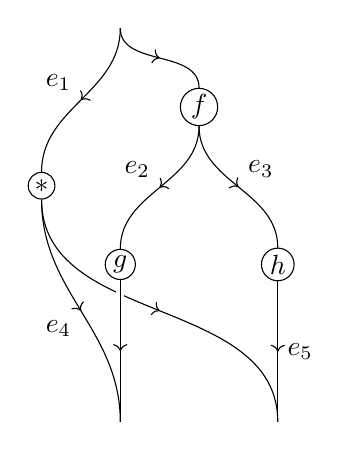
\begin{tikzpicture}
    \node[vertex] (r) at (0,0) {$\ast$};
    \node[vertex] (f) at (2,1) {$f$};
    \node[vertex] (g) at (1,-1) {$g$};
    \node[vertex] (h) at (3,-1) {$h$};
    \draw[edge] (1,2) to[out=-90,in=90] (f);
    \draw[edge] (1,2) to[out=-90,in=90] node[auto,swap] {$e_1$} (r);
    \draw[edge] (r) to[out=-90,in=90] (3,-3);
    \draw[edge] (h) to[out=-90,in=90] node[auto] {$e_5$} (3,-3);
    \draw[cross] (g) to[out=-90,in=90] (1,-3);
    \draw[edge] (g) to[out=-90,in=90] (1,-3);
    \draw[edge] (r) to[out=-90,in=90] node[auto,swap] {$e_4$} (1,-3);
    \draw[edge] (f) to[out=-90,in=90] node[auto,swap] {$e_2$} (g);
    \draw[edge] (f) to[out=-90,in=90] node[auto] {$e_3$} (h);
  \end{tikzpicture}
  \qquad
  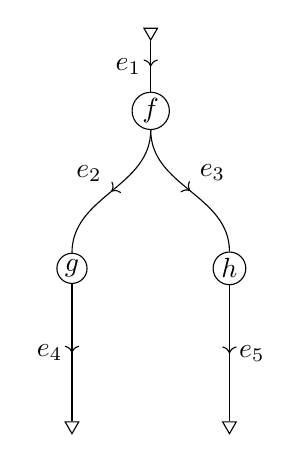
\begin{tikzpicture}
    \node[outer] (e1) at (2,2) {};
    \node[vertex] (f) at (2,1) {$f$};
    \node[vertex] (g) at (1,-1) {$g$};
    \node[vertex] (h) at (3,-1) {$h$};
    \node[outer] (e4) at (1,-3) {};
    \node[outer] (e5) at (3,-3) {};
    \draw[edge] (e1) to[out=-90,in=90] node[auto,swap] {$e_1$} (f);
    \draw[edge] (h) to[out=-90,in=90] node[auto] {$e_5$} (e5);
    \draw[edge] (g) to[out=-90,in=90] node[auto,swap] {$e_4$} (e4);
    \draw[edge] (f) to[out=-90,in=90] node[auto,swap] {$e_2$} (g);
    \draw[edge] (f) to[out=-90,in=90] node[auto] {$e_3$} (h);
  \end{tikzpicture}\label{eq:rooted-graph}
\end{equation}
we think of the edge $e_1$ as ``incoming to the graph'' and the edges $e_4,e_5$ as ``outgoing from the graph'', as drawn above on the right.

Note that an edge like $e_1$ that is ``incoming to the graph'' is \emph{incoming} to the root (as well as to other vertices like $f$), and one like $e_4$ or $e_5$ that is ``outgoing from the graph'' is \emph{outgoing} from the root (as well as from other vertices such as $g$ or $h$).
This choice, which as we will see makes the definition of insertion somewhat simpler, is only possible when using \emph{hyper}graphs, where edges can be incoming to multiple vertices and outgoing from multiple vertices.

% \begin{defn}\label{defn:loop}
%   A \textbf{loop} in a directed hypergraph is a sequence of flags
%   \[(f_0,g_0,f_1,g_1,\dots,f_n,g_n),\]
%   for $n\ge 0$, such that
%   \begin{enumerate}
%   \item Each $f_i,g_i$ are incident on the same edge, and
%   \item Each $g_i,f_{i+1}$ (including $g_n,f_0$ by mod-$n$ arithmetic) are incident on the same vertex, with $g_i$ incoming and $f_{i+1}$ outgoing.
%   \end{enumerate}
%   In particular, a loop with $n=0$ is an edge that is both incoming and outgoing to the same vertex.
%   A directed hypergraph is \textbf{loop-free} if it contains no loops.
% \end{defn}

% The left-hand rooted graph in~\eqref{eq:rooted-graph} is loop-free, which makes sense when considering the right-hand ``graph with free flags'' that it represents.
% If we chose to represent edges ``incoming to the graph'' by edges \emph{outgoing} to the root, then we would have to represent the right-hand ``graph with free flags'' in~\eqref{eq:rooted-graph} by the following rooted graph:
% \begin{equation}
%     \begin{tikzpicture}
%     \node[vertex] (r) at (0,0) {$\ast$};
%     \node[vertex] (f) at (2,1) {$f$};
%     \node[vertex] (g) at (1,-1) {$g$};
%     \node[vertex] (h) at (3,-1) {$h$};
%     \draw[edge] (r) to[out=90,in=90] node[auto] {$e_1$} (f);
%     \draw[edge] (h) to[out=-90,in=-90,looseness=2] node[auto] {$e_5$} (r);
%     \draw[edge] (g) to[out=-90,in=-90] node[auto,very near start] {$e_4$} (r);
%     \draw[edge] (f) to[out=-90,in=90] node[auto,swap] {$e_2$} (g);
%     \draw[edge] (f) to[out=-90,in=90] node[auto] {$e_3$} (h);
%   \end{tikzpicture}\label{eq:loop}
% \end{equation}
% which is not loop-free according to \cref{defn:loop} as written; thus we would have had to special-case the root vertex in \cref{defn:loop}.
% In fact, we regard~\eqref{eq:loop} as representing the following ``graph with free flags'':
% \begin{equation}
%   \begin{tikzpicture}
%     \node[vertex] (f) at (2,1) {$f$};
%     \node[vertex] (g) at (1,-1) {$g$};
%     \node[vertex] (h) at (3,-1) {$h$};
%     \draw[edge] (1,2) to[out=-90,in=90] (f);
%     \draw[edge] (1,2) to[out=-90,in=90] node[auto,swap,near end] {$e_1$} (-1,-4);
%     \draw[edge] (5,3) to[out=-90,in=90] node[auto] {$e_5$} (3,-3);
%     \draw[edge] (h) to[out=-90,in=90] (3,-3);
%     \draw[edge] (g) to[out=-90,in=90] (1,-3);
%     \draw[cross] (-1,3) to[out=-90,in=90] (1,-3);
%     \draw[edge] (-1,3) to[out=-90,in=90] node[auto,swap,near start] {$e_4$} (1,-3);
%     \draw[edge] (f) to[out=-90,in=90] node[auto,swap] {$e_2$} (g);
%     \draw[edge] (f) to[out=-90,in=90] node[auto] {$e_3$} (h);
%   \end{tikzpicture}\label{eq:loops2}
% \end{equation}
% in which $e_4$ and $e_5$ are ``incoming to the graph'' and $e_1$ is ``outgoing from the graph''.
% We do want to consider~\eqref{eq:loops2} as containing ``loops'', because there are paths from ``in'' to ``out'' that travel some paths ``backwards''.\fxnote{Is that right?}

Note also that we allow edges that are not adjacent to any vertices, or that are adjacent to only one vertex, but are \emph{not} adjacent to the root and hence not ``incoming'' or ``outgoing'' to the graph.
The following example shows a number of distinct degenerate possibilities in a directed hypergraph (where $\ast$ is the root):
\begin{center}
  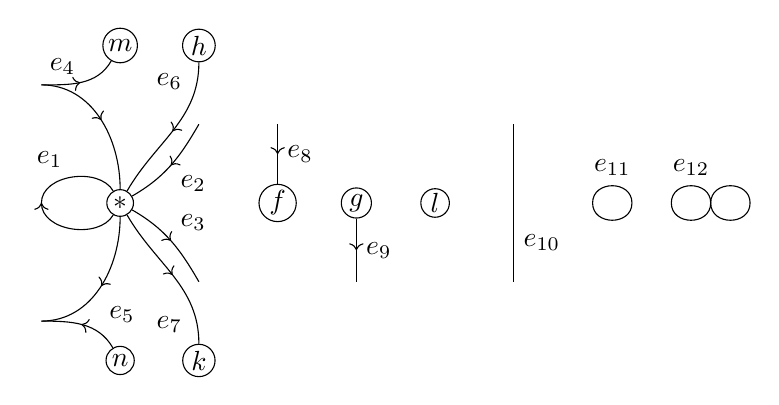
\begin{tikzpicture}
    \node[vertex] (r) at (0,0) {$\ast$};
    \draw[edge] (r) to[out=-120,in=-90] +(-1,0) to[out=90,in=120] node[auto] {$e_1$} (r);
    \draw[edge] (1,1) to[out=-120,in=30] node[auto] {$e_2$} (r);
    \draw[edge] (r) to[out=-30,in=120] node[auto] {$e_3$} (1,-1);
    \node[vertex] (h) at (1,2) {$h$};
    \draw[edge] (h) to[out=-90,in=60] node[auto,swap,near start] {$e_6$} (r);
    \node[vertex] (k) at (1,-2) {$k$};
    \draw[edge] (r) to[out=-60,in=90] node[auto,swap,near end] {$e_7$} (k);
    \node[vertex] (m) at (0,2) {$m$};
    \draw[edge] (-1,1.5) to[out=0,in=-120] node[auto,near start] {$e_4$} (m);
    \draw[edge] (-1,1.5) to[out=0,in=90] (r);
    \node[vertex] (n) at (0,-2) {$n$};
    \draw[edge] (n) to[out=120,in=0] node[auto,swap,near start] {$e_5$} (-1,-1.5);
    \draw[edge] (r) to[out=-90,in=0] (-1,-1.5);
    \node[vertex] (f) at (2,0) {$f$};
    \draw[edge] (2,1) -- node[auto] {$e_8$} (f);
    \node[vertex] (g) at (3,0) {$g$};
    \draw[edge] (g) -- node[auto] {$e_9$} +(0,-1);
    \node[vertex] (l) at (4,0) {$l$};
    \draw (5,1) -- node[auto,near end] {$e_{10}$} (5,-1);
    \draw (6.5,0) to[out=90,in=90,looseness=1.5] node[auto,swap] {$e_{11}$} (6,0) to[out=-90,in=-90,looseness=1.5] (6.5,0);
    \draw (7.5,0) to[out=90,in=90,looseness=1.5] node[auto,swap] {$e_{12}$} (7,0) to[out=-90,in=-90,looseness=1.5] (7.5,0);
    \draw (7.5,0) to[out=90,in=90,looseness=1.5] (8,0) to[out=-90,in=-90,looseness=1.5] (7.5,0);
  \end{tikzpicture}
\end{center}
Here $e_{10}$, $e_{11}$, and $e_{12}$ are all edges not adjacent to any vertices, with genera 0, 1, and 2 respectively.
We did not draw any arrows on them because only flags, not edges, are directed as ``incoming'' or ``outgoing''.
When interpreted as incoming or outgoing to the entire graph, the edges $e_1$--$e_7$ adjacent to the root above would be drawn as follows (preserving the ordering on incoming and outgoing edges to the root by drawing the incoming and outgoing edges to the graph in the same order).
\begin{center}
  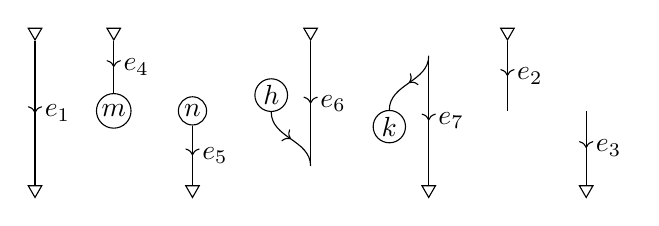
\begin{tikzpicture}
    \node[outer] (e1a) at (2,1) {};
    \node[outer] (e1b) at (2,-1) {};
    \draw[edge] (e1a) -- node[auto] {$e_1$} (e1b);
    \node[outer] (e2) at (8,1) {};
    \draw[edge] (e2) -- node[auto] {$e_2$} (8,0);
    \node[outer] (e3) at (9,-1) {};
    \draw[edge] (9,0) -- node[auto] {$e_3$} (e3);
    \node[vertex] (m) at (3,0) {$m$};
    \node[outer] (e4) at (3,1) {};
    \draw[edge] (e4) -- node[auto] {$e_4$} (m);
    \node[vertex] (n) at (4,0) {$n$};
    \node[outer] (e5) at (4,-1) {};
    \draw[edge] (n) -- node[auto] {$e_5$} (e5);
    \node[vertex] (h) at (5,.2) {$h$};
    \node[outer] (e6) at (5.5,1) {};
    \draw[edge] (e6) -- node[auto] {$e_6$} (5.5,-.7);
    \draw[edge] (h) to[out=-90,in=90]  (5.5,-.7);
    \node[vertex] (k) at (6.5,-.2) {$k$};
    \node[outer] (e7) at (7,-1) {};
    \draw[edge] (7,.7) -- node[auto] {$e_7$} (e7);
    \draw[edge] (7,.7) to[out=-90,in=90] (k);
  \end{tikzpicture}
\end{center}

We note that there are many ways in which a hypergraph can have nontrivial automorphisms.
One simple example is the graph with two vertices and no edges:
\begin{center}
\begin{tikzpicture}
  \node[circle,fill,inner sep=1pt] at (0,0) {};
  \node[circle,fill,inner sep=1pt] at (1,0) {};
\end{tikzpicture}
\end{center}
in which the two vertices can be swapped by an automorphism.
However, it is not necessary to be disconnected to have nontrivial automorphisms:
\begin{center}
  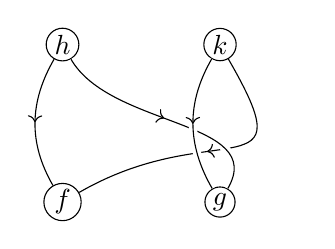
\begin{tikzpicture}[scale=2]
    \node[vertex] (f) at (0,0) {$f$};
    \node[vertex] (g) at (1,0) {$g$};
    \node[vertex] (h) at (0,1) {$h$};
    \node[vertex] (k) at (1,1) {$k$};
    \draw[edge] (h) to[out=-120,in=120] (f);
    \draw[edge] (k) to[out=-60,in=30,looseness=2] (f);
    \draw[cross] (h) to[out=-60,in=60] (g);
    \draw[edge] (h) to[out=-60,in=60] (g);
    \draw[cross] (k) to[out=-120,in=120] (g);
    \draw[edge] (k) to[out=-120,in=120] (g);
  \end{tikzpicture}
\end{center}
Here there is an automorphism that swaps $f$ with $g$ and swaps $h$ with $k$.
Moreover, if we orient this graph by giving the edges the left-to-right ordering in the picture, then this automorphism preserves the orientation.
This example cannot be rooted (the automorphism has no fixed points) --- or more precisely, it cannot occur in the connected component of the root --- but if we use edges that are incident on more than two vertices then we can have nontrivial automorphisms with fixed points:
\begin{center}
  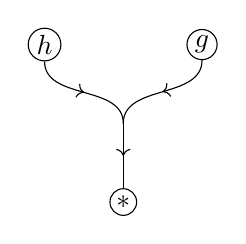
\begin{tikzpicture}
    \node[vertex] (f) at (0,0) {$\ast$};
    \node[vertex] (g) at (1,2) {$g$};
    \node[vertex] (h) at (-1,2) {$h$};
    \draw[edge] (g) to[out=-90,in=90] (0,1);
    \draw[edge] (h) to[out=-90,in=90] (0,1);
    \draw[edge] (0,1) -- (f);
  \end{tikzpicture}
\end{center}
Here there is an automorphism that swaps $g$ and $h$ and fixes the root $\ast$.
The most restrictive thing we can say about about automorphisms is:

\begin{lem}
  A connected rooted directed binary hypergraph has no nontrivial automorphisms.
\end{lem}
\begin{proof}
  Suppose $\phi$ is an automorphism.
  By assumption, it must preserve the root.
  Since it is locally-ordered, it must preserve all edges adjacent to the root.
  But since each of those edges is adjacent to exactly one other vertex, it must preserve those vertices too.
  Proceeding inductively we find that it must preserve all edges and vertices in the connected component of the root, which is all of them since the graph is connected.
\end{proof}

The presence of nontrivial automorphisms means that in general, we cannot simply ``pass to isomorphism classes'' of hypergraphs, and thus structures over hypergraphs are not definable using ``set-based shapes'', such as polynomial monads on the category of polygraphs.
In~\cite{bb:htapm} isomorphism classes and polynomial monads are shown to work for certain subclasses of graphs, but even when it works such a restriction is technical and error-prone.
Thus, we will generally work instead with categories and groupoids, never passing to isomorphism classes, and using a pseudomonad rather than a strict one.

We end this section by comparing our graphs to others in the literature.
Graphs with ``free flags'' have been used in defining many kinds of operads, but usually only in a ``non-hyper'' version, corresponding to non-cartesian operads.
The corresponding restriction in our theory is the following:

\begin{defn}
  A hypergraph is \textbf{binary}, or simply a \textbf{graph}, if % for each edge $e$ we have
  % \[ \rank(e) + 2 \cdot \genus(e)  = 2, \]
  % i.e.\ if
  every edge either has rank 2 and genus 0, or rank 0 and genus 1.
\end{defn}

Amusingly, this condition can be reformulated by saying that the rank of an edge is the same as its ``Euler characteristic'' $\chi=2-2g$.
Its directed version is a little kludgy to state due to our convention about the orientations of flags adjacent to the root.

\begin{defn}
  A \textbf{directed rooted binary hypergraph} is a hypergraph that is separately directed, rooted, and binary, and moreover if we switched the direction of all flags adjacent to the root, then every edge would have equal in-rank and out-rank.
\end{defn}

In a binary rooted hypergraph, we can define an involution on the set of flags not adjacent to the root by sending each flag to the other flag of its corresponding edge, if that flag is not adjacent to the root, or to itself otherwise.
The quotient of this involution is then isomorphic to the set of edges that are adjacent to some non-root vertex.
Thus, we can equivalently define a binary rooted hypergraph by giving
\begin{itemize}
\item a set $F$ of flags (the flags not adjacent to the root),
\item an involution on $F$,
\item a set of ``exceptional linear edges'' (the edges adjacent to the root twice),
\item a set of ``exceptional loops'' (the edges not adjacent to any vertex --- the only ones with genus 1), and
\item a set $V$ of (non-root) vertices and a function $F\to V$ with finite linearly ordered fibers (equivalently, a ``partition'' of $F$ into finite linearly ordered blocks, some of which are allowed to be empty).
\end{itemize}
This is the definition of ``graph'' used commonly in operad theory, e.g.~\cite{bm:gen-opds,km:gwcqceg,costello:ainf,mms:wheeled-props,gk:modular-operads}, although often exceptional loops and edges are omitted or treated inconsistently.

Alternatively, if we remove the root but not the flags adjacent to it, then the function $F\to V$ becomes a partial function, which is defined on a flag just when that flag is not adjacent to the root.
Now we still have the exceptional edges (those adjacent to two flags that are not adjacent to any vertices) and the exceptional loops (those not adjacent to any flags).
This is essentially how binary rooted hypegraphs are encoded in~\cite{bb:htapm}, except that their exceptional loops are ``adjacent to a single flag twice'' rather than to no flags at all.

Another possibility is to express the partial function $F\rightharpoonup V$ as a relation, i.e.\ a span $F \ot H \to V$ in which $H\to F$ is injective.
If we exclude the possibility of exceptional loops, then the function $F\to E$ is a 2-to-1 surjection and hence can be encoded up to isomorphism by a fixed-point-free involution of $F$.
This is the definition of graph from~\cite{jk:feynman} (though they call the elements $H$ the ``flags'' and those of $F$ the ``(directed) edges'').
Their graph morphisms are similar to ours, although theirs are not required to preserve the ``degree of the root''.


\section{Type theory for hypergraphs}
\label{sec:tt-hy}

For all of this section let $P$ be a fixed polygraph.
We will describe a type theory for $P$-labeled hypergraphs; this includes unlabeled hypergraphs as the degenerate case when $P$ is terminal.

An \textbf{edge context} $\Delta$ is a finite list of distinct variables, each labeled with an object of $P$ as its type.

\begin{mathpar}
  \inferrule{ }{\ec \edgectx}
  \and
  \inferrule{\Delta\edgectx \\ p\in P \\ x\notin \Delta}{(\Delta,x:p) \edgectx}
\end{mathpar}

A \textbf{loop context} $\Xi$ in an edge context $\Delta$ is a finite list of equalities between variables of the same type.

\begin{mathpar}
  \inferrule{ }{\Delta \types \ec\loopctx}
  \and
  \inferrule{\Delta\types\Xi\loopctx \\ (x:p)\in \Delta \\ (y:p)\in\Delta}{\Delta\types (\Xi,x\doteq y) \loopctx}
\end{mathpar}

A \textbf{vertex} in an edge context is a morphism of $P$ with variables of appropriate type assigned as its domain and codomain.

\begin{mathpar}
  \inferrule{\alpha\in P(p_1,\dots,p_n;q_1,\dots,q_m) \\ (x_i\in p_i)\in\Delta \\ (y_j\in q_j)\in\Delta}{\Delta \types \alpha(x_1,\dots,x_n;y_1,\dots,y_m) \vertex}
\end{mathpar}

A \textbf{graph context} is an edge context, a loop context, and a finite list of variables assigned to vertices.

\begin{mathpar}
  \inferrule{\Delta \edgectx \\ \Delta\types \Xi\loopctx}{\Delta \mid\Xi\types \ec\graph}
  \and
  \inferrule{\Delta \mid\Xi\types \Gamma\graph \\ \Delta\types M\vertex \\ (f\notin \Gamma)}{\Delta\mid\Xi\types (\Gamma,f:M)\graph}
\end{mathpar}

\begin{thm}
  A graph context determines, and is determined by, a finite $P$-labeled hypergraph $\G\to P$.
\end{thm}
\begin{proof}
  The variables in the edge context correspond to the set of objects of the edge groupoid $E$, and their assignment to types is the action of  $\G\to P$ on edges.
  The equalities in the loop context correspond to freely generating isomorphism in the edge groupoid $E$.
  The variables in the graph context correspond to the vertices, and their type assignment to a morphism of $P$ is the action of $\G\to P$ on vertices.
  Finally, the list of variables in a syntactic vertex $\alpha(x_1,\dots,x_n;y_1,\dots,y_m)$ specifies the flags.
\end{proof}

I'm not sure in what sense we can say this is an equivalence.
Maybe we shouldn't even try at this point.

In particular, note that self-equalities $(x\doteq x)$ in the loop context correspond to automorphisms in the groupoid $E$, hence to edges of nontrivial genus.
Thus, it is only reasonable to simplify by substituting along equalities of \emph{distinct} variables:
\begin{equation}\label{eq:subst}
  \inferrule{\Delta,y:p\mid\Xi,x\doteq y \types \Gamma\graph \\ x\not\jdeq y}{\Delta\mid\Xi[x/y]\types \Gamma[x/y] \graph}
\end{equation}
This should change the corresponding hypergraph into an \emph{equivalent} one by contracting an object along an isomorphism.


\section{Insertion of hypergraphs}
\label{sec:insertion}

We now define an operation of \emph{insertion} of hypergraphs, which replaces some of the vertices in one graph by entire new graphs having the same ``flag structure''.
Suppose $\G = (V\ot F \to E)$ is a hypergraph, and for some subset $V_0 \subseteq V$ and each $v\in V_0$ we have a rooted hypergraph $\H_v = (V_v \ot F_v \to E_v)$ whose root $\ast_v$ has the same degree as $v$.
In the directed case, we require it to have the same in-degree and out-degree separately.
(Usually, $V_0$ will be either a single vertex or the set of all non-root vertices.)
There is a unique induced order-preserving (and, in the directed case, direction-preserving) bijection between the flags adjacent to $v$ and the flags adjacent to $\ast_v$, yielding a pair of pullback squares
\[
\begin{tikzcd}
  F \ar[d] & F_0 \ar[l] \dlpullback \ar[d] \ar[r] \drpullback & \sum_v F_v \ar[d]\\
  V & V_0 \ar[l] \ar[r] & \sum_v V_v
\end{tikzcd}
\]
where the map $V_0 \to \sum_v V_v$ sends $v$ to $\ast_v$.

We define the \textbf{insertion} of the $\H_v$'s into $\G$ at the vertices $v\in V_0$, denoted 
\[ \ins{\G}{V_0}{v}{\H_v} \]
to be obtained by first taking the pseudo-pushout of the following hypergraphs (which exists since $F_0$ is a discrete set):
\[
\begin{tikzcd}
  E & F_0 \ar[d,equals] \ar[r] \ar[l] & \sum_v E_v & E' & E' \ar[l,equals]  \\
  F \ar[d] \ar[u] & F_0 \ar[l] \dlpullback \ar[d] \ar[r] \drpullback & \sum_v F_v \ar[d] \ar[u] &
  F' \ar[u] \ar[d] & F' \setminus F_0 \ar[l] \ar[d] \ar[u] \dlpullback \\
  V & V_0 \ar[l] \ar[r] & \sum_v V_v & V' & V' \setminus V_0 \ar[l]
\end{tikzcd}
\]
and then removing all the vertices coming from $V_0$ and the flags adjacent to them (those in $F_0$), as shown by the pullback on the right above.
Explicitly, this means:
\begin{itemize}
\item A vertex in $V'$ is either a non-root vertex of some $V_v$, or a vertex in $V\setminus V_0$.
\item A flag in $F'$ is either a flag in some $F_v$ not adjacent to the root, or a flag in $F$ not adjacent to a vertex in $V_0$.
  % Because $\mathbf{Set}$ is an adhesive category~\cite{ls:adhesive},
  The flags adjacent to a vertex coming from $V_v$ or $V$ are precisely those adjacent to it in $F_v$ or $F$ respectively.
  % In particular, the insertion hypergraph is naturally locally-ordered and directed if the inputs are.
\item An edge in $E'$ is either an edge in some $E_v$ or an edge in $E$, where an edge in $E_v$ adjacent to the root $\ast_v$ is identified with the corresponding edge adjacent to $v$ in $E$.
\end{itemize}
\fxnote{Add some examples.}

To make it easier to prove abstract properties of insertion, we identify the last ``removing vertices'' step using a factorization system and a ``relational composition''.

\begin{thm}
  There is a bicategorical unique factorization system on $\hy$, in which the left class $\L$ consists of morphisms that are bijective on vertices (hence also on flags) and the right class $\R$ consists of morphisms that are an equivalence on groupoids of edges.
  Moreover, both classes of maps are preserved by the pseudo-pushouts from \cref{thm:pushout}.
\end{thm}
\begin{proof}
  Any map factors as an $\L$-map followed by an $\R$-map:
  \[
  \begin{tikzcd}
    V' \ar[d,equals] & F' \ar[l] \ar[d,equals] \dlpullback \ar[r] & E' \ar[d] \\
    V' \ar[d] & F' \ar[l] \ar[d] \ar[r] \dlpullback & E \ar[d,equals]\\
    V & F \ar[l] \ar[r] & E
  \end{tikzcd}
  \]
  and it is easy to see that this factorization is unique up to equivalence.
  The last statement follows since the pseudo-pushouts are constructed using pushouts of sets and pseudo-pushouts of groupoids, which preserve bijections and equivalences respectively.
\end{proof}

A \textbf{corolla} is a hypergraph of the form $1 \ot F = F$, i.e.\ having one vertex, each flag of which is adjacent to a unique edge.
A disjoint union of corollas, i.e.\ a hypergraph of the form $V \ot F = F$, is called an \textbf{inflorescence}.\footnote{A corolla is the whorl of petals in a flower; an inflorescence is a cluster of flowers on a single stem.}

\begin{thm}
  There is a tricategory $\hyrel$, which in fact is a bicategory enriched over 2-categories, in which:
  \begin{itemize}
  \item The objects are finite inflorescences.
  \item The morphisms are cospans $\A \to \G \ot \B$ of finite hypergraphs such that $(\A+\B) \to \G$ is bijective on vertices.
  \item The composite of $\A \to \G \ot \B$ and $\B \to \H \ot \C$ is given by taking the pseudo-pushout $\G +_{\B} \H$ and then $(\L,\R)$-factoring the induced map $(\A + \C) \to (\G +_{\B} \H)$.
  \item The unit of an inflorescence $\A$ is given by $(\L,\R)$-factoring the codiagonal $(\A+\A)\to\A$.
  \end{itemize}
\end{thm}
\begin{proof}
  It is classical to construct the bicategory of relations (jointly monic spans) in any regular category, with composition defined by pullback followed by (strong epi, mono) factorization.
  More generally, this works using any pullback-stable factorization system.
  The present theorem is a bicategorical version of the dual of that result; a similar construction is used in~\cite{cjsv:modulated-bicats}.

  We can make it very explicit (and see the strictness) as follows: first define a tricategory whose objects are finite sets and whose hom-2-categories are cospans with vertex a groupoid.
  Composition is by pseudo-pushout, and it is easy to see that when we use pseudo-pushouts that have a strict 2-categorical universal property this operation is associative up to isomorphism (not just equivalence).
  In this way we get a bicategory enriched over 2-categories.

  Now a finite inflorescence is determined by a map of sets $F\to V$ with finite linearly ordered fibers, and a cospan as in the theorem statement is then determined by a cospan $F_1 \to E \ot F_2$ with $E$ a suitable groupoid.
  Thus, our desired structure is obtained by adding extra ignored structure to the objects of this 2-category-enriched bicategory (the objects $V$ with maps from $F$) and restricting its hom-2-categories (to require finitely-generated freeness of the automorphism groups).
\end{proof}

Now, if $\G= (V\ot F\to E)$ is any hypergraph and $V_0$ is a subset of its vertices, with $F_0$ the pullback of $F$ to $V_0$, then we can define
\begin{align*}
  \G|_{V_0} &= (V_0 \ot F_0 = F_0)\\
  % \G_{F_0} &= (\emptyset \ot \emptyset \to F_0)\\
  \G|_{\neg V_0} &= ((V\setminus V_0) \ot (F\setminus F_0) = (F\setminus F_0))
\end{align*}
and regard $\G$ as a morphism from $\G|_{V_0}$ to $\G|_{\neg V_0}$ in $\hyrel$.
Similarly, if $\H$ is a rooted hypergraph, we can regard it as a morphism from $\H|_{\neg \ast}$ to $\H|_\ast$ in $\hyrel$.
Thus, if for each $v\in V_0$ we have a rooted hypergraph $\H_v$ whose root has the same degree as $v$, then $\sum_v \H_v|_\ast \cong\G|_{V_0}$.
Inspecting the definition of insertion, we have:

\begin{thm}
  The insertion $\ins{\G}{V_0}{v}{\H_v}$ is the composite of the morphisms
  \[
  \begin{tikzcd}
    \textstyle \sum_v \H|_{\neg \ast} \ar[r,"\mathclap\circ" description,"\sum_v \H_v"] &
    \sum_v \H_v|_\ast \cong\G|_{V_0} \ar[r,"\mathclap\circ" description,"\G"] &
    \G|_{\neg V_0}
  \end{tikzcd}
  \]
  in $\hyrel$.\qed
\end{thm}

This makes it easy to show that insertion of hypergraphs is coherently associative in an appropriate sense.

\begin{thm}\label{thm:ins-assoc}
  Suppose we have
  \begin{itemize}
  \item a hypergraph $\G$,
  \item a subset $V_0$ of vertices in $\G$,
  \item for each $v\in V_0$ a rooted hypergraph $\H_v$ whose root $\ast_v$ has the same degree as $v$,
  \item for each $v$ a subset $W_v$ of non-root vertices in $\H_v$, and
  \item for each $v$ and $w\in W_v$ a rooted hypergraph $\K_w$ whose root $\ast_w$ has the same degree as $w$.
  \end{itemize}
  Then there is an isomorphism:
  \begin{equation}
    \ins{\Bigl(\ins{\G}{V_0}{v}{\H_v}\Bigr)}{\sum_v W_v}{w}{\K_w} \;\cong \;
    \ins{\G}{V_0}{v}{\Bigl(\ins{\H_v}{W_v}{w}{\K_w}\Bigr)}\label{eq:ins-assoc}
  \end{equation}
  If moreover we also have
  \begin{itemize}
  \item for each $v$ and $w$ a subset $U_w$ of non-root vertices in $\K_w$, and
  \item For each $v,w$ and $u\in U_w$ a rooted hypergraph $\L_u$ whose root $\ast_u$ has the same degree as $u$,
  \end{itemize}
  then the following pentagon commutes:
  \[
  \begin{tikzcd}
    ((\G \insy \H_v)\insy \K_w)\insy \L_u \ar[rr,"\cong"] \ar[d,"\cong"'] &&
    (\G \insy (\H_v\insy \K_w))\insy \L_u \ar[d,"\cong"] \\
    (\G\insy \H_v) \insy (\K_w \insy \L_u) \ar[dr,"\cong"'] && \G\insy ((\H_v \insy \K_w) \insy \L_u) \ar[dl,"\cong"]\\
    & \G \insy (\H_v \insy (\K_w \insy \L_u))
  \end{tikzcd}
  \]
\end{thm}
\begin{proof}
  The isomorphism~\eqref{eq:ins-assoc} is just an instance of the associativity isomorphism for $\hyrel$, and similarly the pentagon is one of its coherence laws.
\end{proof}

Similarly, insertion is unital in an appropriate sense.
Let $\C_n$ denote the rooted $n$-corolla, which has $n$ edges of genus 0 and two vertices $c$ and $\ast$ (the root) each adjacent to all of them in the same order.

\begin{thm}\label{thm:ins-unit}
  If $\G$ is any hypergraph with a subset $V_0$ of vertices, then
  \[ \ins{\G}{V_0}{v}{\C_{\degree(v)}} \;\cong\; \G.\]
  Similarly, if $\G$ is any rooted hypergraph whose root has degree $n$, then
  \[ \ins{\C_n}{}{c}{\G} \;\cong\; \G. \]
  Finally, if $\G$ is any hypergraph with a subset $V_0$ of vertices, and for each $v\in V_0$ we have a rooted hypergraph $\H_v$ whose root has the same degree as $v$, then the following triangle commutes:
  \[
  \begin{tikzcd}
    (\G \insy \C_{\degree(v)} ) \insy \H_v \ar[rr,"\cong"] \ar[dr,"\cong"'] &&
    \G \insy (\C_{\degree(v)} \insy \H_v) \ar[dl,"\cong"] \\
    & \G \insy \H_v
  \end{tikzcd}
  \]
\end{thm}
\begin{proof}
  As before, this is just a unit isomorphism and coherence law for $\hyrel$, noting that the \emph{rooted} $n$-corolla $\C_n$ is the unit morphism in $\hyrel$ for the \emph{unrooted} $n$-corolla.
\end{proof}

\cref{thm:ins-assoc,thm:ins-unit} are also true in the directed case.
To see this, we can just work in the slice 2-category over $\dhy$, using the fact that pseudo-colimits in any slice 2-category are created in the base.

\section{Type theory for insertion}
\label{sec:tt-insertion}

In type theory it is easiest to describe insertion when $V_0$ is a single vertex.
We represent a rooted hypergraph as a graph context together with another vertex judgment in the same edge/loop context.
The fact that two vertices have the same degree is automatic when in the labeled case they have the same label.
This leads to the following insertion/substitution (admissible) rule:

\begin{mathpar}
  \inferrule{\Delta_1\mid\Xi_1 \types \Gamma_1 \graph\\
    \Delta_1\mid\Xi_1 \types \alpha(\vec x;\vec y)\vertex \\
    \Delta_2\mid\Xi_2 \types \Gamma_2, \alpha(\vec u;\vec v) \graph}
  {\Delta_1,\Delta_2 \mid \Xi_1,\Xi_2, \vec x\doteq \vec u, \vec y \doteq \vec v \types \Gamma_1, \Gamma_2 \graph}
\end{mathpar}

The equalities $\vec x\doteq \vec u, \vec y \doteq \vec v$ correspond to the isomorphisms inserted by the pseudo-pushout of groupoids.
We are assuming $\Delta_1\cap \Delta_2=\emptyset$, so all of these are equalities between distinct variables, and thus at least some of them can be substituted away by~\eqref{eq:subst} (a ``unification algorithm'' for the arguments of the two $\alpha$-labeled vertices).
However, we may still be left with additional self-loops, for instance:

\begin{mathpar}
  \inferrule*{\inferrule*{x:p \mid\cdot \types \Gamma_1 \graph\\
    x:p \mid\cdot \types \alpha(x,x;) \vertex \\
    u:p \mid\cdot \types \Gamma_2, \alpha(u,u;) \graph}
  {x:p,u:p \mid x\doteq u, x\doteq u \types \Gamma_1,\Gamma_2\graph}}
{x:p \mid x\doteq x \types \Gamma_1,\Gamma_2[x/u] \graph}
\end{mathpar}


\section{The pseudomonad for hypercategories}
\label{sec:hypercats}

Let \cpg be the 2-category of \textbf{\Cat-polygraphs}, i.e.\ internal polygraphs in \Cat, or equivalently internal categories in polygraphs.
Thus a \Cat-polygraph has a category $P(0)$ of objects together with, for each $n,m\in\N$, a category $P(n,m)$ of $n$-ary $m$-coary morphisms, equipped with $n+m$ functors $P(n,m) \to P(0)$.
We may regard an ordinary polygraph as a discrete \Cat-polygraph.
\fxnote{How does this categorical direction interact with the groupoid direction in $E$?}

A \textbf{bracketing} of $n$ things is a list of natural numbers whose sum is $n$, regarded as as giving the number of things in each bracket.
The \textbf{arity} of the bracketing is the length of the list.
For instance, the bracketing $(2,0,3,1)$ of $6$, of arity $4$, should be thought of as $(xx)()(xxx)(x)$.

A \textbf{bracketed hypergraph} is a rooted locally-ordered directed hypergraph together with bracketings of the incoming and outgoing edges at the root.
An isomorphism of bracketed hypergraphs must, of course, preserve the bracketings.
If the incoming and outgoing bracketings have arities $n$ and $m$ respectively, we call it an $(n,m)$-bracketed hypergraph.

If $G$ is a rooted hypergraph, we write $G_0$ for the result of removing the root and all flags adjacent to it (but not removing any edges).
If $k\in\N$, we write $\mathbf{k}$ for the polygraph with $n$ objects (i.e.\ edges) and no morphisms (i.e.\ vertices), hence no flags.
If $G$ is an $(n,m)$-bracketed hypergraph, then we have $n+m$ polygraph morphisms $\mathbf{k}\to G_0$, as $k$ varies over the numbers in the bracketings, which are pairwise disjoint and together enumerate the edges adjacent to the root, grouped according to the specified bracketing.

Now, given a \Cat-polygraph $P$, define a new \Cat-polygraph $T P$ as follows.
\begin{enumerate}
\item The category of objects $T P(0)$ is the free strict monoidal category on the category of objects $P(0)$.
  Thus its objects and arrows are finite lists of those in $P(0)$.
  Equivalently, its objects are \Cat-polygraph maps $\mathbf{k}\to P$ for some $k\in\N$, and its arrows are natural transformations (2-cells in \cpg)
  \[
  \begin{tikzcd}
    \mathbf{k} \ar[rr,equals] \ar[dr] & ~ \ar[d,phantom,"\Rightarrow"] & \mathbf{k} \ar[dl] \\ & P
  \end{tikzcd}
  \]
\item The objects of $TP(n,m)$ are morphisms of polygraphs $G_0\to P$, where $G$ is an $(n,m)$-bracketed hypergraph.
  An arrow in $TP(n,m)$ from $G_0\to P$ to $H_0\to P$ consists of an equivalence of $(n,m)$-bracketed hypergraphs $G\cong H$ together with a transformation
  \[
  \begin{tikzcd}
    G_0 \ar[rr,"\cong"] \ar[dr] & ~ \ar[d,phantom,"\Rightarrow"] & H_0 \ar[dl] \\ & P
  \end{tikzcd}
  \]
\item The $n+m$ functors $TP(n,m) \to TP(0)$ are obtained by precomposing with the $n+m$ polygraph morphisms $\mathbf{k}\to G_0$ described above.
  These morphisms commute with any isomorphism of bracketed hypergraphs, so this precomposition acts on arrows as well as on objects.
\end{enumerate}

\begin{lem}
  This defines a 2-functor $T:\cpg\to\cpg$ that preserves connected limits and groupoidal objects.
\end{lem}
\begin{proof}
  Functoriality is easy by postcomposition.
  If $P = \lim P_i$ is a connected limit, then an object or arrow of $\lim T P_i(0)$ must have the same $\mathbf{k}$ everywhere and hence lift uniquely to an element of $T P(0)$.
  Similarly, the $G$ and $H$ must be constant for any object or arrow $\lim T P_i(n,m)$ so that it lifts uniquely to $T P (n,m)$.
  Finally, it is clear from the definition that if all arrows in $P$ are invertible, the same is true for $TP$.
\end{proof}

Let $\C_{n,m}$ denote the rooted $(n,m)$-corolla:
\begin{center}
  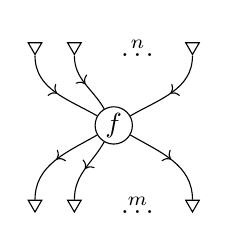
\begin{tikzpicture}
    \node[outer] (a1) at (-1,1) {};
    \node[outer] (a2) at (-.5,1) {};
    \node at (0.3,1) {$\overset{n}{\dots}$};
    \node[outer] (an) at (1,1) {};
    \node[vertex] (f) at (0,0) {$f$};
    \node[outer] (b1) at (-1,-1) {};
    \node[outer] (b2) at (-.5,-1) {};
    \node at (0.3,-1) {$\overset{m}{\dots}$};
    \node[outer] (bn) at (1,-1) {};
    \draw[edge] (a1) to[out=-90,in=150] (f);
    \draw[edge] (a2) to[out=-90,in=120] (f);
    \draw[edge] (an) to[out=-90,in=30] (f);
    \draw[edge] (f) to[out=-150,in=90] (b1);
    \draw[edge] (f) to[out=-120,in=90] (b2);
    \draw[edge] (f) to[out=-30,in=90] (bn);
  \end{tikzpicture}
\end{center}
This is an $(n,m)$-bracketed hypergraph with exactly one non-root vertex and with bracketings $n=\overbrace{1+1+\cdots+1}^n$ and $m=\overbrace{1+1+\cdots+1}^m$.
For any polygraph $P$, morphisms $(C_{n,m})_0 \to P$ are in bijection with vertices of $P$ having in-degree $n$ and out-degree $m$.

Now, for any polygraph $P$, we define $\eta_P : P \to T P$ as follows:
\begin{enumerate}
\item $\eta:P(0) \to TP(0)$ sends an object $x\in P(0)$ to its classifying map $x:\mathbf{1}\to P$, and similarly on arrows.
\item $\eta:P(n,m) \to TP(n,m)$ sends an object $f\in P(n,m)$ to its classifying map $f:(C_{n,m})_0\to P$, and similarly on arrows.
\end{enumerate}

\begin{thm}
  This defines a fully faithful cartesian 2-natural transformation $\eta: 1\to T$.
\end{thm}
\begin{proof}
  Naturality is easy, since postcomposing classifying maps is the same as acting on objects and arrows.
  Full faithfulness on $0$-parts is easy, while on $(n,m)$-parts it follows from the fact that $C_{n,m}$ has no nontrivial automorphisms.
  Finally, $\eta$ is cartesian, meaning that its naturality squares are pullbacks, since its image consists precisely of the objects and arrows involving $\mathbf{1}$ or $C_{n,m}$.
\end{proof}

Of course, there are many different (isomorphic) $(n,m)$-corollas.
However, the theorem is true as long as we fix a \emph{particular} such corolla for each $(n,m)$ to use in defining $\eta$.
The existence of other corollas means that $\eta$, though fully faithful, is not replete: objects of $TP$ defined using other corollas are isomorphic to ones in the image of $\eta$ but are not in the image of $\eta$ themselves.

Using insertion of hypergraphs, we define a cartesian 2-natural transformation $\mu:T^2\to T$.
\fxnote{Incomplete}

However, the monad laws hold only up to coherent isomorphism, so that we have a ``cartesian pseudomonad'' of a fairly strict sort (the functor and transformations are strict and strictly cartesian; only the monad laws are pseudo).
\fxnote{Incomplete}

\begin{defn}
  A $T$-pseudoalgebra is called a \textbf{double hypercategory}.
\end{defn}

A double hypercategory $H$ has the following structure:
\begin{itemize}
\item A set of \emph{objects}, the objects of the category $H(0)$.
\item A set of \emph{vertical arrows}, the arrows of $H(0)$, which can be composed in the usual way.
\item An (unbiased, non-strict) monoidal structure on the category of objects and vertical arrows.
\item For each $n,m$, a set of \emph{horizontal arrows} with lists of $n$ objects as source and $m$ objects as target (the objects of the category $H(n,m)$).
\item For each $n,m$, a set of \emph{2-cells} with horizontal arrows as ``vertical source and target'', and lists of $n$ vertical arrows and $m$ vertical arrows as ``horizontal source and target''.
  These can be composed vertically.
\item ``Horizontal composition'' operations on horizontal arrows and 2-cells, parametrized by bracketed hypergraphs.
  That is, if we label the non-root vertices of any rooted locally-ordered directed hypergraph by horizontal arrows of $H$, in such a way that the edges are labeled compatibly by objects, and bracket the incoming and outgoing edges to the root, then we obtain a composed horizontal arrow whose source and target are obtained by applying the monoidal structure on objects to the groups in the brackets.
  We can similarly compose hypergraphs labeled by 2-cells, and this operation is functorial with respect to vertical composition.
\item Moreover, isomorphisms of bracketed hypergraphs induce isomorphisms of composed horizontal arrows, naturally.
  In particular, this applies to \emph{automorphisms}.
\end{itemize}

\begin{defn}
  If a double hypercategory has only identity vertical arrows, we call it a \textbf{2-hypercategory}.
  If it additionally has only identity 2-cells, we call it a \textbf{hypercategory}.%
  \footnote{The word ``hypercategory'' was also used by~\cite{hmt:strict-n-hypercats,mt:omega-hypergraphs}.
    Our meaning is somewhat different, but not unrelated since they also use a kind of hypergraph.
    The ``hyperstructures'' of~\cite{baas:higher-structures} are also related, although in contrast to both of these references we consider here only one dimension of hyper-dependency.}
\end{defn}

\begin{eg}
  Let \bC be a symmetric monoidal category in which every object is equipped with the structure of a Frobenius algebra (but we do \emph{not} assume that all morphisms of \bC are monoid or comonoid homomorphisms).
  Then \bC has the structure of a hypercategory.
  In fact, it could be that this is exactly what a hypercategory is.
\end{eg}

\begin{eg}
  More generally, a sufficiently strictly monoidal 2-category in which every object has the structure of a Frobenius pseudomonoid~\cite{street:frob-psmon} gives rise to a 2-hypercategory.
  In particular, this applies to any cartesian bicategory~\cite{ckww:cartbicats-ii} in which every object is Frobenius~\cite{ww:frob-cart} and in which the monoidal structure is strict enough.

  In general, what can we take the vertical arrows to be?
  Arbitrary left adjoints?
  Morphisms that are colax for both monoid and comonoid structures?
\end{eg}

\begin{eg}
  If \bS has finite products, then an \bS-indexed monoidal category with indexed homotopy coproducts preserved by the tensor product on both sides, in the sense of~\cite{ps:indexed}, gives rise to a double hypercategory whose vertical category is \bS.
\end{eg}




\section{Virtual double hypercategories}
\label{sec:vdhc}

Our main purpose in defining the pseudomonad $T$ was to consider $T$-multicategories.
Leinster~\cite{leinster:higher-opds} defines $T$-multicategories with respect to a cartesian monad on any category with pullbacks.
Here we have only a pseudomonad on \cpg, but this causes little difficulty, especially since we are interested in the ``object-discrete'' case.

\begin{defn}
  A \textbf{virtual double hypercategory} $M$ consists of the following.
  \begin{enumerate}
  \item A polygraph $M_0$.
  \item A discrete fibration of \Cat-polygraphs $M_1 \to M_0 \times TM_0$.
  \item A composition operation $M_1 \times_{TM_0} TM_1 \to M_1$ over $1\times \mu$:
    \[
    \begin{tikzcd}
      M_1 \times_{TM_0} TM_1 \ar[r,dashed] \ar[d] & M_1\ar[d]\\
      M_0 \times TTM_0 \ar[r,"1\times \mu"'] & M_0\times TM_0.
    \end{tikzcd}
    \]
  \item A unit $M_0 \to M_1$ over $(1,\eta)$:
    \[
    \begin{tikzcd}
      M_0 \ar[r,dashed] \ar[d,equals] & M_1 \ar[d] \\
      M_0\ar[r,"{(1,\eta)}"'] & M_0\times TM_0.
    \end{tikzcd}
    \]
  \item An associativity isomorphism lying over the pseudomonad coherence isomorphism:
    \[\hspace{-2cm}
    \begin{tikzcd}
      & M_1 \times_{TM_0} TM_1 \ar[drr] \ar[ddd]\\
      M_1 \times_{TM_0} TM_1 \times_{TTM_0} TTM_1 \ar[ur] \ar[drr] \ar[ddd] \ar[rrr,phantom,"\cong"] &&&
      M_1 \ar[ddd] \\
      && M_1 \times_{TM_0} TM_1  \ar[ur]\ar[ddd]\\
      & M_0\times TTM_0\ar[drr] \\
      M_0 \times TTTM_0 \ar[ur] \ar[drr] \ar[rrr,phantom,"\cong"] &&&
      M_0\times TM_0 \\
      && M_0\times TTM_0\ar[ur]
    \end{tikzcd}\hspace{-2cm}
    \]
  \item Unit isomorphisms lying over the pseudomonad coherence isomorphisms:
    \[
    \begin{tikzcd}
      & M_1 \times_{TM_0} TM_1 \ar[dr] \ar[dddr,phantom,"\cong" very near start] \ar[dd] \\
      M_1 \ar[rr,equals] \ar[ur]\ar[dd] &~ & M_1\ar[dd]\\
      & M_0\times TM_0 \times TTM_0 \ar[dr] \ar[d,phantom,"\cong"] \\
      M_0\times TM_0 \ar[rr,equals]\ar[ur] &~& M_0\times TM_0
    \end{tikzcd}
    \]
    (There are two such isomorphisms, but the pictures look the same except that the omitted labels on the arrows should be different.)
  \end{enumerate}
\end{defn}

Since $M_1 \to M_0\times TM_0$ is assumed to be a discrete fibration, the coherence isomorphisms are unique, and automatically satisfy any axioms we might wish them to; thus we do not bother writing down those axioms (which would simply lift the corresponding pseudomonad axioms).
Explicitly, a virtual double hypercategory has the following structure.

\begin{enumerate}
\item A set of \emph{objects} (the objects of $M_0$).
\item A set of \emph{vertical multi-arrows}, with source a finite list of objects and target a single object (the objects of $M_1$).
  These can be composed as in an ordinary (non-symmetric) multicategory.
\item For each $n,m$, a set of \emph{horizontal arrows} with lists of $n$ objects as source and $m$ objects as target (the morphisms in the polygraph $M_0$).
\item A set of \emph{2-cells}, each of which has a bracketed hypergraph labeled by horizontal arrows as its vertical source, a single horizontal arrow as its vertical target, and lists of vertical multi-arrows as its horizontal source and target.
\item Each horizontal arrow has an identity 2-cell.
\item A composition operation on 2-cells that involves hypergraph insertion, which is appropriately associative and unital.
\end{enumerate}

We also have algebras over generalized multicategories, for which again we restrict to the discrete case.
Here there is no room for nontrivial isomorphisms at all.

\begin{defn}
  If $M$ is a virtual double hypercategory, an \textbf{$M$-algebra} consists of the following.
  \begin{enumerate}
  \item A polygraph $A$ with a map $A \to M_0$.
  \item An action map $M_1 \times_{TM_0} TA \to A$ over $M_0$.
  \item The action is associative and unital:
    \[\hspace{-2cm}
    \begin{tikzcd}
      M_1 \times_{TM_0} TM_1 \times_{TTM_0} TTA \ar[r] \ar[d] &M_1 \times_{TM_0} TA \ar[d]\\
      M_1 \times_{TM_0} TA \ar[r] & A
    \end{tikzcd}
    \qquad
    \begin{tikzcd}
      A \ar[r] \ar[dr,equals] & M_1 \times_{TM_0} TA\ar[d] \\ & A
    \end{tikzcd}\hspace{-2cm}
    \]
  \end{enumerate}
\end{defn}


\section{Undirected hypercategories and kits}
\label{sec:kits}

Can define similar monad using undirected hypergraphs.
The virtual undirected ones are a special case of directed virtual ones in which all sources are empty.
Kits should be a virtual undirected ones living over a ``shape'' one that marks variance.


\section{Type theory of virtual double hypercategories}
\label{sec:type-theory}

We adopt a ``type-theoretic rule'' notation for 2-cells in virtual double hypercategories.
To describe a labeled hypergraph, we assign a variable to each edge, and declare the variables as having the corresponding objects as ``types'' with their genera as annotations on the typing declaration, for instance
\begin{mathpar}
  x :^0 p \and y:^1 p \and z:^0 q
\end{mathpar}
where $p,q,r$ are objects of $M$.
In practice the genera will almost always be $0$, in which case we omit to notate them.
We notate the vertices as sequents with their labeling horizontal arrow as a term, and with their incident edges as the input and output variables:
\begin{mathpar}
  (x,y,x) \types \alpha: (x,z) \and
  (z,z,y) \types \beta:()
\end{mathpar}
Thus, we must have $\alpha:(p,p,p) \to (p,q)$ and $\beta : (q,q,p) \to ()$.
These declarations all occur in the ``premises''.
Finally, we treat vertical multi-arrows as function symbols and ``apply'' them to the variables denoting the corresponding edges, then place the resulting terms in a ``conclusion'' sequent, labeled again by a horizontal arrow:
\begin{mathpar}
  (F(x,y),x) \types \gamma : (z,G())
\end{mathpar}
For vertical identity arrows, we simply write the variable itself, i.e.\ $x$ means $1_p(x)$ and $z$ means $1_q(z)$.
If $F:(p,p)\to q$ and $G:() \to p$, then we must have $\gamma : (q,p) \to (q,p)$.
Putting the above examples together, we obtain the rule
\begin{mathpar}
  \inferrule{x :^0 p \\ y:^1 p \\ z:^0 q \\
    (x,y,x) \types \alpha: (x,z) \\ (z,z,y) \types \beta:()}
  {(F(x,y),x) \types \gamma : (z,G())}
\end{mathpar}
which corresponds to the following graphically drawn 2-cell:
\begin{center}
  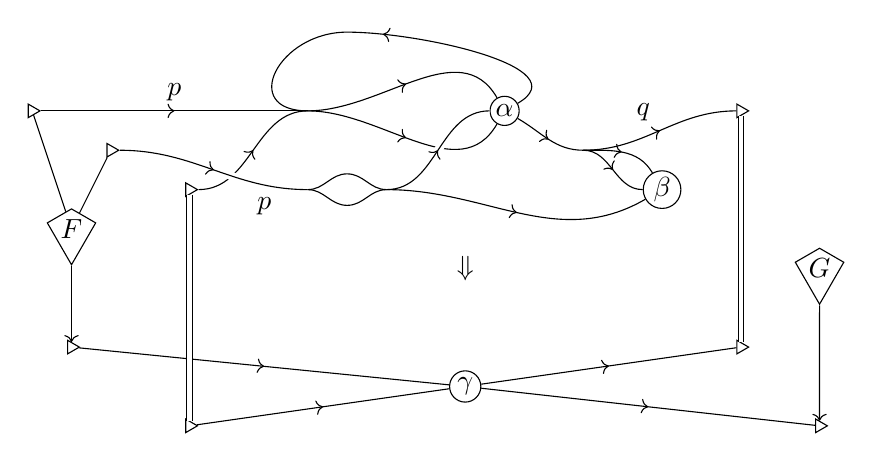
\begin{tikzpicture}
    \node[houter] (Fxy) at (.5,0) {};
    \node[houter] (idx) at (2,-1) {};
    \node[vertex] (gm) at (5.5,-.5) {$\gamma$};
    \node[houter] (idz) at (9,0) {};
    \node[houter] (G) at (10,-1) {};
    \draw[edge] (Fxy) -- (gm);
    \draw[edge] (idx) -- (gm);
    \draw[edge] (gm) -- (idz);
    \draw[edge] (gm) -- (G);
    \node[kite,draw,inner sep=1pt] (Gin) at (10,1) {$G$};
    \draw[->] (Gin) -- (G);
    \node[houter] (zout) at (9,3) {};
    \draw[double,double equal sign distance] (zout) -- (idz);
    \node[houter] (xin) at (2,2) {};
    \draw[double,double equal sign distance] (xin) -- (idx);
    \node[houter] (xyinx) at (0,3) {};
    \node[houter] (xyiny) at (1,2.5) {};
    \node[kite,draw,inner sep=1pt] (F) at (.5,1.5) {$F$};
    \draw (xyinx) -- (F);
    \draw (xyiny) -- (F);
    \draw[->] (F) -- (Fxy);
    \node[vertex] (be) at (8,2) {$\beta$};
    \node[vertex] (al) at (6,3) {$\alpha$};
    \coordinate (x) at (3.5,3);
    \coordinate (y) at (3.5,2);
    \draw[edge] (xyinx) to[out=0,in=180] node[auto] {$p$} (x);
    \draw[edge] (xin) to[out=0,in=180] (x);
    \draw[cross] (xyiny) to[out=0,in=180] (y);
    \draw[edge] (xyiny) to[out=0,in=180] node[auto,swap,very near end] {$p$} (y);
    \draw[edge] (x) to[out=0,in=120] (al);
    \draw[edge] (x) to[out=0,in=-120] (al);
    \coordinate (y2) at (4.5,2);
    \draw[cross] (y2) to[out=0,in=-180] (al);
    \draw[edge] (y2) to[out=0,in=-180] (al);
    \draw (y) to[out=0,in=180] (4,2.2) to[out=0,in=180] (y2);
    \draw (y) to[out=0,in=180] (4,1.8) to[out=0,in=180] (y2);
    \draw[edge] (al) to[out=30,in=0] (4,4) to[out=180,in=180,looseness=2] (x);
    \coordinate (z) at (7,2.5);
    \draw[edge] (al) to[out=-30,in=180] (z);
    \draw[edge] (z) to[out=0,in=120] (be);
    \draw[edge] (z) to[out=0,in=180] (be);
    \draw[edge] (y2) to[out=0,in=-150] (be);
    \draw[edge] (z) to[out=0,in=-180] node[auto] {$q$} (zout);
    \node at (5.5,1) {$\Downarrow$};
  \end{tikzpicture}
\end{center}

Identity 2-cells are easy:
\[ \inferrule{ (x,y,z) \types \alpha : (u,v,w) }{ (x,y,z) \types \alpha : (u,v,w) }\]
Composition of 2-cells is, thankfully, well-notated by combining rules in derivation trees, and \emph{substituting} the terms such as $F(x,y)$ in the conclusion of one rule into the variables occurring in the premises of another.
We do have to be careful that the vertical arrow parts match up between all the 2-cells we are precomposing with.
\fxnote{Some examples?}

It is important to note that when we write a 2-cell as a ``rule'' we are not ``deriving the conclusion from the premises''.
Instead each ``rule'' is a datum, namely the 2-cell, and putting together rules into derivation trees is an operation on these data.

When we get to \emph{$M$-algebras}, however, the rules become operations on sequents.
Here we notate the objects lying over an object $p$ by
\[A \type_p \qquad\text{or}\qquad A_p,\]
and the morphisms lying over $\alpha : (p,q,r) \to (u,v)$ by
\[(A_p,B_q,C_r) \types_\alpha f : (D_u,E_v).\]
Now the 2-cell considered above \emph{acts} on morphisms in the algebra, which we can interpret as a rule of the usual sort that produces a conclusion from the premises:
\begin{mathpar}
  \inferrule{A \type_p \\ B \type^1_p \\ C \type_q \\\\
    (A,B,A) \types_\alpha f : (A,C) \\ (C,C,B) \types_\beta g :()}
  {(F(A,B),A) \types_\gamma g\circ_\rho f : (C,G())}
\end{mathpar}
where $g\circ_\rho f$ denotes a sort of ``composition'' of $f$ and $g$ parametrized by the rule $\rho$.
Note that the vertical arrows $F$ and $G$ act similarly on \emph{types}, which we can notate with type formation rules:
\begin{mathpar}
  \inferrule{A\type_p \\ B\type_p}{F(A,B) \type_q}
  \and
  \inferrule{ }{G() \type_p}
\end{mathpar}

In this way, we can interpret a virtual double hypercategory as a reasonably general sort of \emph{specification of a sequent calculus}.
The objects are the \emph{modes} to which the types can belong.
The horizontal arrows are the \emph{mode morphisms}, or \emph{sequent forms}.
The vertical arrows are the \emph{type formation rules}.
And the 2-cells are the \emph{derivation rules} for sequents.
Each derivation rule takes as premises some number of types, each with a specified mode, and some number of sequents containing those types, each with a specified form, and yields as a conclusion a sequent with a specified form containing some of the types from the premises together with potentially other new types formed from them by the formation rules.
We call this a ``sequent calculus'' because the type formation operators can only appear in the conclusion; all types in the premises must be (meta-)variables.

Note that all the contraction, weakening, composition, and identities are performed formally in the vertical domain.
We contract two types by making the corresponding flags incident on the same edge, and so on.
In the type-theoretic notation, this is indicated by using the same (meta-)variable for the types in the corresponding places.
Even the symmetric action (exchange) is performed formally in the domain, since the incoming and outgoing edges on the root are ordered, and the vertical multi-arrows preserve ordering --- but this ordering is not visible in the premises of the type-theoretic notation, instead being indicated by the order in which the (meta-)variables appear in the conclusion.

The fact that vertical arrows and 2-cells have an algebraic structure of composition means that all \emph{derivable} rules are present on an equal footing with the primitive ones, along with all equations that hold between such derivations.
The primitive rules and primitive equality axioms between composites of these form a \emph{presentation} of a virtual double hypercategory by generators and relations.


\section{Examples}
\label{sec:examples}

For now, we consider only examples without type formation rules.

\subsection{Intuitionistic type theories}
\label{sec:intuitionistic}

We obtain intuitionistic type theories simply by requiring all mode morphisms to have unary targets.
If we have one mode $p$ and one such morphism $p^n \to p$ for each $n$, we can express the identity and cut rules of ordered logic:
\begin{mathpar}
  \inferrule{A\type}{A\types A}
  \and
  \inferrule{\Gamma\types A \\ \Delta,A,\Psi\types B}{\Delta,\Gamma,\Psi\types B}
\end{mathpar}
We can assert axioms on the composites of these to obtain the semantic structure of a non-symmetric multicategory.

We can then add the exchange rule of intuitionistic linear logic:
\begin{mathpar}
  \inferrule{\Gamma,A,B,\Delta\types C}{\Gamma,B,A,\Delta\types C}
\end{mathpar}
with axioms yielding a symmetric multicategory.

\subsection{Flavors of operad}
\label{sec:operads}

All of these use only binary directed graphs.
A summary is in~\cite{bb:htapm}.

Directed sorts:
\begin{itemize}
\item Wheeled props~\cite{mms:wheeled-props} use arbitrary directed graphs.
\item Props use directed graphs with no directed loops.
\item Properads~\cite{vallette:properads} use connected directed graphs with no directed loops.
\item Wheeled properads use arbitrary connected directed graphs.
\item Dioperads~\cite{gan:dioperads} / polycategories~\cite{szabo:polycats,koslowski:polycats,garner:polycats} have no directed loops and are connected and simply connected (no undirected loops either), or equivalently contractible.~\cite{markl:operads-props}
\item Symmetric operads/multicategories use arbitrary directed trees.
\item Non-symmetric operads/multicategories use planar directed trees.
\end{itemize}

Undirected sorts:
\begin{itemize}
\item Cyclic operads~\cite{gk:cyclic-operads} use undirected trees; compare to~\cite{co:flang-cyclic}.
\item Modular operads~\cite{gk:modular-operads} use arbitrary connected graphs (plus a ``stability'' condition).
\item Compact symmetric multicategories~\cite{jk:feynman} use arbitrary graphs.
  This is a somewhat misleading name as it doesn't indicate that the objects are actually \emph{self-}dual (the undirectedness).
\end{itemize}

\bibliography{../all.bib}
\bibliographystyle{alpha}

\end{document}
